\documentclass[a4paper,12pt]{article}
\usepackage{graphicx,textcomp,amsmath,amssymb,IEEEtrantools,adjustbox,wrapfig,chngcntr,tikz,float,amsthm,listings,caption,enumitem,caption,subcaption,siunitx,booktabs,multirow,array,cancel}
\usepackage[toc,page]{appendix}

%BACKLINK SETUP FOR CLICKABLE LINKS
\usepackage{hyperref}
\hypersetup{
    colorlinks,
    citecolor=blue,
    filecolor=blue,
    linkcolor=blue,
    urlcolor=blue
}
%END-BACKLINK SETUP FOR CLICKABLE LINKS

\usepackage{pgfplots}


\usepackage{parskip}
\usepackage{indentfirst}

\usepackage{fancybox} 


\definecolor{codegreen}{rgb}{0,0.6,0}
\definecolor{codegray}{rgb}{0.5,0.5,0.5}
\definecolor{codepurple}{rgb}{0.58,0,0.82}
\definecolor{backcolour}{rgb}{0.95,0.95,0.92}

%WHEN DOES EQUATION COUNTER CHANGE
\counterwithin{equation}{section}
%END-WHEN DOES EQUATION COUNTER CHANGE

%DOUBLE SPACING IF NEEDED
\usepackage{setspace}
\onehalfspacing
%END-DOUBLE SPACING IF NEEDED


%BORDER
\usepackage[paperwidth=7.27in,paperheight=10.69in,left=0.5in, right=0.5in, top=1in, bottom=1in]{geometry}
\usepackage[a4,frame,center,noinfo]{crop}
%END-BORDER

\usepackage{fancyhdr}
\pagestyle{fancy}
\fancyhead{}
\renewcommand{\headrulewidth}{0pt}
\usepackage{blindtext}
\usepackage{lastpage}
\rfoot{Page{} \thepage\ of \pageref{LastPage}}
\cfoot{}
\chead{\footnotesize{Multivariable optimization using the Cobb-Douglas function}}



%PARAGRAPH INDENTATION
\setlength{\parskip}{1em}
\setlength{\parindent}{1cm}
%END-PARAGRAPH INDENTATION

\binoppenalty=10000
\relpenalty=10000

\newtheorem{theorem}{Theorem}
\theoremstyle{definition}
\newtheorem{definition}{Definition}

\begin{document}

%TITLE PAGE
%\begin{titlepage}
%    \begin{center}
%    
%        \vspace*{0.2cm}
% 
%        \Large
%        \textbf{Mathematics Exploration}
%        
% 		\textbf{Higher Level}
%
%        
%
%        \vspace{2.5cm}
%		
%		
%		\textbf{Exploration Title: }Multivariable optimization using the Cobb-Douglas function
% 
%        \vfill
% 
% 
%        \vspace{0.8cm}
%
% 
%    \end{center}
%\end{titlepage}

\usetikzlibrary{positioning}

\usetikzlibrary{arrows}



\section{Introduction and personal engagement}
The age-old question every mathematician turned economist has asked is, how do I maximize production? Or more commonly, how do I minimize costs?

As both a mathematics and economics student for the last 4 years, I have often wondered about the relationships between these two disciplines. In my Theory of Knowledge classes, I was able to further examine their relationship as Areas of Knowledge. I quickly realized that economics often is the practical application of mathematics. My interest in the application of mathematics to economics has only been fueled by my father, who is an entrepreneur for numerous companies. He told me economists often use mathematical equations to model how certain phenomenon function, as well as depict  economic activities such as production, supply, demand, and costs. 

One such function is the Cobb-Douglas function which represents the relationship between two or more inputs and the output produced\footnote{Coma, Charles W., and Paul H. Douglas. ``A theory of production." \textit{Proceedings of the Fortieth Annual Meeting of the American Economic Association,} vol. 139., 1928.\label{ref:cobbd}}.

Thus, I commenced an investigation on \textbf{how to maximize the production, and minimize the cost for firms where they factors of production are represented by the Cobb-Douglas Function.} My father provided me with real data from one of his business ventures to aid me in my goal.  

\subsection{Cobb-Douglas Function}\label{sec:cobbd}
A Cobb-Doulas production function is a function which takes on the following form\textsuperscript{\ref{ref:cobbd}},

\begin{equation}\label{eq:cobbd}
		f(L,K)=Q=A \cdot L^m \cdot K^n
\end{equation}
Where equation \eqref{eq:cobbd} is true if $A,m,n>0$. While the technical economic definitions are unnecessary for this investigation it is important to know what each variable stands for. $Q$ is the total production (real values of all good produced in an year), $L$ is labor input (the number of hours worked by people in an year),  $K$ is the capital input (the value of the capital divided by its price, to show its utility),  $A$ is a constant, and $m$ and $n$ are constants of the output elasticities of labour and capital respectively (the change in output from a change in input, determined by the responsiveness to change of the factors of production).

\section{Mathematical investigation}
\subsection{Raw Data}
The dataset below was provided to me by my father and is of real companies he works with. With this data, the parameters of the Cobb-Douglas function (elaborated in section \ref{sec:cobbd}) can be estimated. The table gives the natural logarithm of the original data as $\ln K$, $\ln L$, and $\ln Q$ which are the natural logs of labor input, capital input, and total production respectively. This is because the Ordinary Least Square (OLS) method cannot be used for datasets in which the independent variable is non-linear\footnote{Amemiya, Takeshi. \textit{Advanced Econometrics.} Harvard University Press, 2001.} . Therefore, transforming the data into natural logarithms makes the independent variables linear, and allows for OLS. The table on the right begins where the table of the left ended.

\setlength{\extrarowheight}{0pt}
\begin{table}[H]
\begin{center}
\begin{tabular}{|lllll|} \toprule
    $\ln K$ &  & $\ln L$ &  & $\ln Q$\\ \midrule

								    3.6889 &       &   3.6889    &       &   3.4675 \\
                                    3.6889 &       &  4.7875     &       &    3.8069 \\
                                    3.6889 &      &   5.2983    &       &     3.7564 \\
                                    3.6889 &       &   5.7683   &       &    4.0918 \\
                                    4.3820 &      &    3.6889   &       &   3.5946 \\ 
                                    4.3820 &      &   4.3820   &      &  3.5149 \\
                                    4.3820 &      &    5.0752   &       &   4.1281 \\
                                    4.3820 &      &    5.6348   &      &    4.4534\\
                                    4.7875 &      &    4.7875   &       &   4.0031 \\
                                    4.7875 &       &    5.2983   &       & 4.1896 \\ 
                                    4.7875 &      &    5.7683   &       &  4.5463\\
                                    5.0752 &      &    3.6889   &      &  3.6430 \\
                                    5.0752 &      &   4.3820    &      &  4.1242 \\
                                    5.0752 &       &    5.0752   &       &   4.4723 \\
                                    5.0752 &       &     5.4806  &      &   4.3563 \\ \bottomrule
\end{tabular}
\quad \quad \quad \quad \quad 
\begin{tabular}{|lllll|} \toprule
    $\ln K$ &  & $\ln L$ &  & $\ln Q$\\ \midrule

								    5.2983 &       &   4.7875    &       &   4.3965 \\
                                    5.2983 &       &  5.2983     &       &    4.3934 \\
                                    5.2983 &      &   5.7683    &       &     4.7487 \\
                                    5.4806 &       &   3.6889  &       &    3.6726 \\
                                    5.4806 &      &    5.0752   &       &   4.4991  \\ 
                                    5.4806 &      &   4.3820   &      &  4.5027  \\
                                    5.4806 &      &    5.6348   &       &   4.6062  \\
                                    5.6348 &      &    4.3820   &      &    4.2190 \\
                                    5.6348 &      &    4.7875   &       &   4.0904  \\
                                    5.6348 &       &    5.4806   &       & 4.7451  \\ 
                                    5.6348 &      &    5.7683   &       &  4.7228 \\
                                    5.7683 &      &    3.6889   &      &  3.9925  \\
                                    5.7683 &      &   4.7875    &      &  4.7719  \\
                                    5.7683 &       &    5.2983   &       &  4.9012  \\
                                    5.7683 &       &     5.7683  &      &   4.8305 \\ \bottomrule
\end{tabular}
\caption{Raw data in natural logarithm form}
\label{tab:rawdata}
\end{center}
\end{table}


\subsection{Estimating Cobb Douglas parameters}
As discussed previously, the raw data in table \ref{tab:rawdata} can be used to estimate the values for the parameters of the Cobb-Douglas function. This will be done through linear regression using the OLS method. From equation \eqref{eq:cobbd} we know that,
\begin{equation}
	Q=AL^mK^n
\end{equation}
Taking log on both sides,
\begin{equation}\label{eq:logcobbd}
	\ln Q=\ln A+ m \ln L + n \ln K
\end{equation}
For the case of this investigation, $y = \ln Q$ will be taken as the dependent variable, and $x= \ln L + \ln K$ will be the independent variable. Firstly, we need to find the regression coefficient which is basically the slope of the graph.


\begin{equation}
	\text{Regression Coefficient = } \beta =\frac{\text{Covariance(X,Y)}}{\text{Variance(X)}}=\frac{COV(X,Y)}{\sigma_X^2}
\end{equation}
\begin{equation}
	\Rightarrow \frac{E(XY)-E(X)E(Y)}{\sigma_X^2}=\frac{\frac{1}{30}\sum\limits_{i=1}^{30}(x_iy_i- \overline{x}\cdot \overline{y}}{\frac{1}{30}\sum\limits_{i=1}^{30}(x_i- \overline{x})^2}
\end{equation}
where the mean of the dependent variable $y$ $=4.241367$ and the standard deviation is $=0.422242$.

Furthermore, we need to calculate the intercept for the regression,
\begin{equation}
	\text{Intercept} = \alpha = \frac{1}{30}\sum^{30}_{i=1}(y_i- \beta x_i)
\end{equation}

Now those are the basics required for OLS regression, we can use the Regression Data Analysis function in Microsoft Excel to get an estimation for all the values\footnote{Jingze, Jiang. ``How to Use Excel to Estimate the Cobb-Douglas Production Function." \textit{YouTube} 17 Apr. 2016, www.youtube.com/watch?v=FYHLc4zhjzg. Accessed on 10 Feb. 2019.} . Solving this regression manually is out of the scope of this investigation.



\begin{table}[H]
\centering
\caption{Regression Statistics}
\begin{tabular}{*2l}
\toprule
\multicolumn{2}{c}{Regression Statistics}\\
\midrule
	Multiple R & 0.935543981 \\ 
	R Square & 0.87524254 \\ 
	Adjusted R Square & 0.866001247 \\ 
	Standard Error & 0.154565081 \\ 
	Observations & 30 \\ 
\bottomrule
\end{tabular}
\end{table}




% Table generated by Excel2LaTeX from sheet 'Sheet2'
\begin{table}[H]
  \centering
  \caption{ANOVA table}
    \begin{tabular}{lrrrrr}
    \toprule
          & \multicolumn{1}{c}{\textit{df}} & \multicolumn{1}{c}{\textit{SS}} & \multicolumn{1}{c}{\textit{MS}} & \multicolumn{1}{c}{\textit{F}} & \multicolumn{1}{c}{\textit{Significance F}} \\
    \midrule
    Regression & 2     & 4.52531097 & 2.26265549 & 94.7099621 & 6.2647E-13 \\
    Residual & 27    & 0.64503983 & 0.02389036 &       &  \\
    Total & 29    & 5.17035081 &       &       &  \\
    \bottomrule
    \end{tabular}%
  \label{tab:anova}%
\end{table}%


% Table generated by Excel2LaTeX from sheet 'Sheet2'
\begin{table}[H]
  \centering
  \caption{Coefficient values}
    \begin{tabular}{lrrrrrr}
    \toprule
          & \multicolumn{1}{c}{\textit{Coefficients}} & \multicolumn{1}{c}{\textit{Std. Error}} & \multicolumn{1}{c}{\textit{t Stat}} & \multicolumn{1}{c}{\textit{P-value}} & \multicolumn{1}{c}{\textit{Lower 95\%}} & \multicolumn{1}{c}{\textit{Upper 95\%}} \\
    \midrule
    Intercept & 0.45000105 & 0.27899655 & 1.61292695 & 0.11838922 & -0.1224526 & 1.02245468  \\
    lnK   & 0.34706602 & 0.04187643 & 8.2878597 & 6.7657E-09 & 0.26114267 & 0.43298936 \\
    lnL   & 0.41448138 & 0.04043764 & 10.2498907 & 8.3391E-11 & 0.3315102 & 0.49745257 \\
    \bottomrule
    \end{tabular}%
  \label{tab:vals}%
\end{table}%

Using these statistics we can estimate the $\ln A$, $m$, and $n$ (given in table \ref{tab:vals}) and plug them into equation \eqref{eq:logcobbd},
\begin{equation}
	\ln Q=0.45000105 +0.34706602 \ln K+ 0.41448138 \ln L
\end{equation}
Obviously these values have a Standard Error associated with them (due to the nature of linear regression), which is the given in the third column of table \ref{tab:vals}.

Furthermore, it gives us the following values for constants,
\begin{equation}
	\begin{split}
		A &= 1.56831 \approx 1.57 \\
		n &= 0.34706602 \approx 0.35 \\
		m &= 0.41448138 \approx 0.41 
	\end{split}
\end{equation}

These values can be said to be statistically significant due to the low $p$-value associated with them. Since both the $p$-value for $\ln K$ and $\ln L$ are 6.7657E-9 and 8.3391E-11 respectively, which are lesser than 0.05, the null hypothesis, or the idea that these values are incorrect, can be rejected.

Now, we can finally convert obtain our Cobb-Douglas function in the same format as equation \eqref{eq:cobbd}

\begin{equation}\label{eq:realcobbd}
	f(L,K)=Q \Rightarrow A \cdot L^m \cdot K^n = 1.57L^{0.41}K^{0.35}
\end{equation}

According to the Cobb-Douglas function if $m+n < 1$, returns of scale are decreasing\footnote{Coma, Charles W., and Paul H. Douglas. ``A theory of production." \textit{Proceedings of the Fortieth Annual Meeting of the American Economic Association,} vol. 139., 1928.}. That means marginal utility (change in utility) as production is increased. Let's see if the optimization matches this prediction.

\begin{figure}[H]
\centering
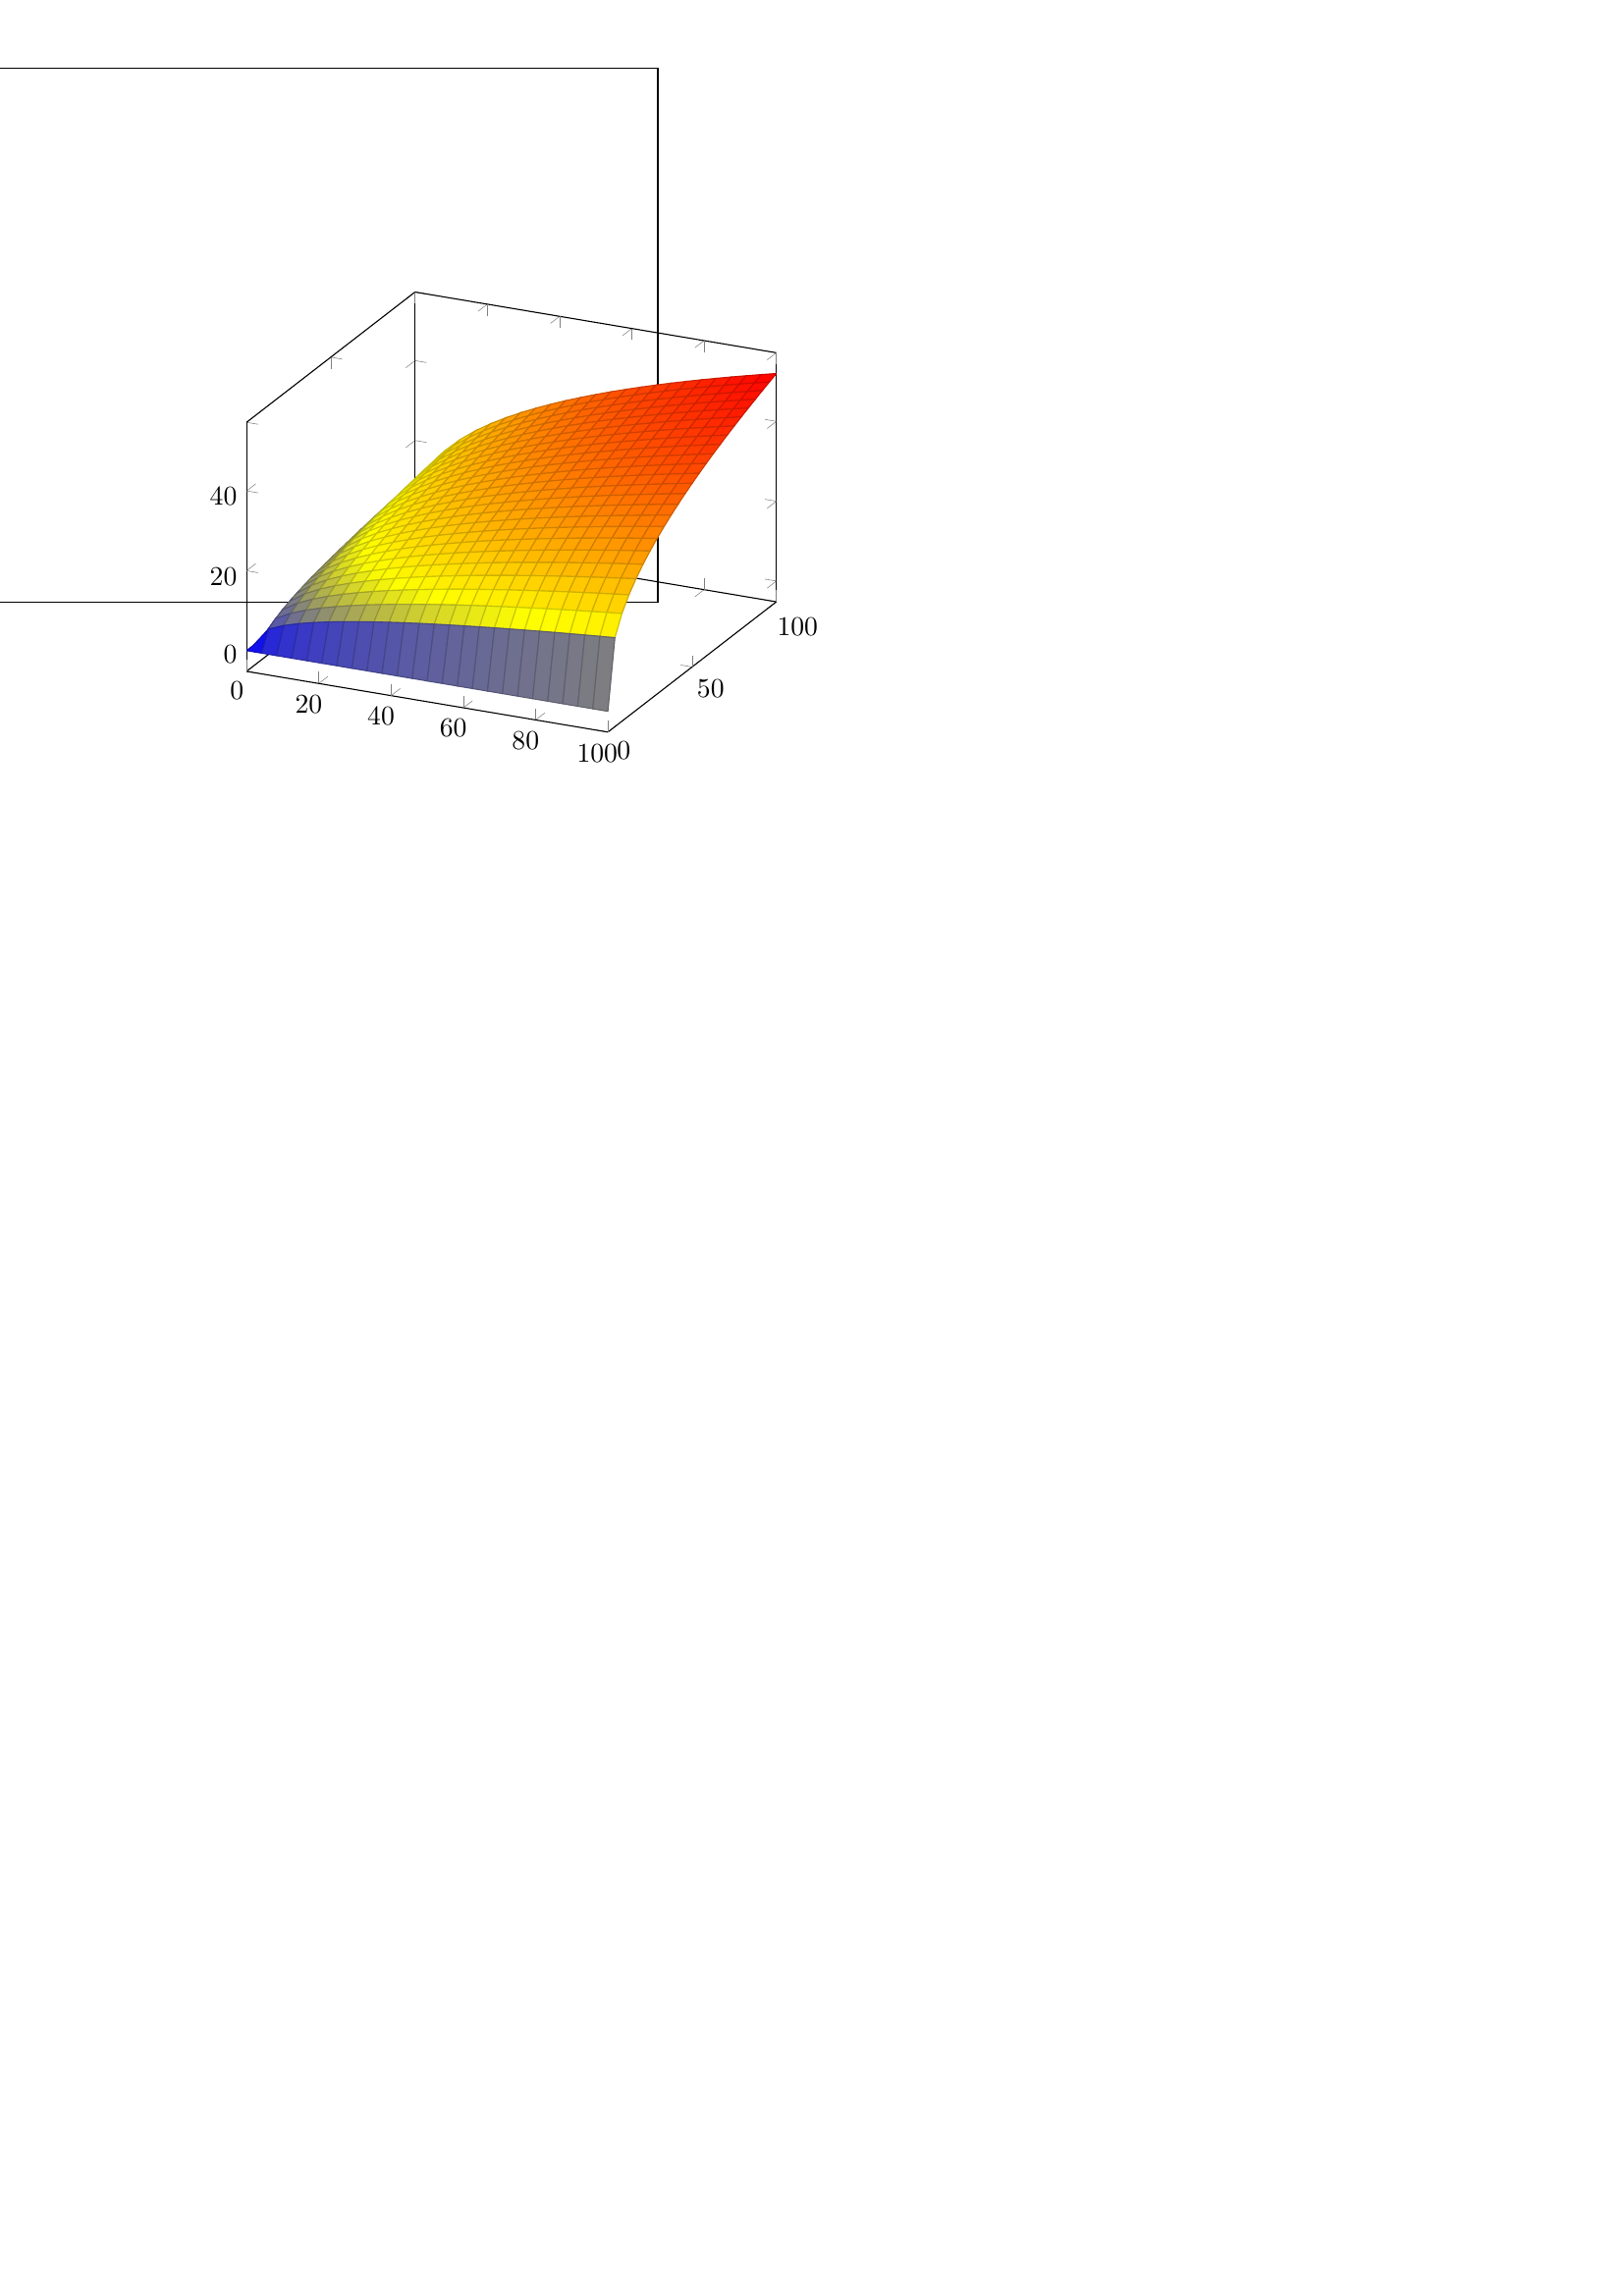
\begin{tikzpicture}
\begin{axis}[domain=0:100,y domain=0:100]
\addplot3[surf]{1.57*x^.41*y^.35};
\end{axis}
\end{tikzpicture}
\caption{$f(L,K)$ graphed}
\end{figure}

\subsection{Optimization of the Cobb-Douglas function}\label{sec:cobbdopt}
When optimizing equation \eqref{eq:realcobbd}, certain labor and capital costs must be taken, as well as a budget to be invested in both. These can be taken as arbitrary for this step.

Let the cost of labor be \$900 per unit

Let the cost of capital be \$1800 per unit

Let the total budget of the be \$1,080,000

Calculating how many units of labor and capital are required to maximize product subject to budgetary constraint,
\begin{equation}
\begin{split}
		900L+1800K &= 108000 \\
		9L+18K &= 10800
\end{split}
\end{equation}

Now, the method of Lagrange Multiplier can be used to maximize $Q$ under this constraint\footnote{Beveridge, G. S. G., and R. S. Schechter. \textit{Optimization: Theory and Practice.} McGraw-Hill, 1970.}.

According to Lagrange Multiplier method, a function $f(L,K)$ is maximized or minimized at $g(L,K)=0$ , that is, when, $\nabla f = \lambda \nabla g$ where $\lambda$ is just some multiple and $\nabla f$,$\nabla g$ are the gradients of $f$ and $g$ respectively. Therefore the constraint can be rewritten as,
\begin{equation}\label{eq:constraint}
	g(L,K)=9L+18K-10800=0
\end{equation}

Giving a system of equations for the partial derivatives of $L$ and $K$ as from equation \eqref{eq:realcobbd},
\begin{equation}\label{eq:partialL}
	P_L=\lambda g_L \Rightarrow \frac{\partial}{\partial L} =  \lambda g_L \Rightarrow 0.6437\cdot L^{-0.59} \cdot K^{0.35} = \lambda \cdot 9
\end{equation}
\begin{equation}\label{eq:partialK}
	P_K = \lambda g_K \Rightarrow \frac{\partial}{\partial K} = \lambda g_K \Rightarrow 0.5495 \cdot K^{-0.65}\cdot L^{0.41} = \lambda \cdot 18
\end{equation}

Now solving equations \eqref{eq:constraint}, \eqref{eq:partialL}, and \eqref{eq:partialK} as a system of equations.

Firstly solving equation \eqref{eq:partialL}, and \eqref{eq:partialK} for $\lambda$,
\begin{equation}\label{eq:lambdaL}
	P_L \Rightarrow \lambda = \frac{0.6437\cdot L^{-0.59} \cdot K^{0.35}}{9}
\end{equation}
\begin{equation}\label{eq:lambdaK}
	P_K \Rightarrow \lambda = \frac{0.5495 \cdot K^{-0.65}\cdot L^{0.41}}{18}
\end{equation}

Equating \eqref{eq:lambdaL} and \eqref{eq:lambdaK},
\begin{equation}
		\frac{0.6437\cdot L^{-0.59} \cdot K^{0.35}}{9} = \frac{0.5495 \cdot K^{-0.65}\cdot L^{0.41}}{18}
\end{equation}
\begin{equation}
		\Rightarrow	1.2874 \cdot L^{-0.59} \cdot K^{0.35} = 0.5495 \cdot K^{-0.65}\cdot L^{0.41}
\end{equation}
\begin{equation}
	\Rightarrow 1.2874 K^{}=0.5495L^{}
\end{equation}
\begin{equation}\label{eq:valueofL}
	\Rightarrow2.3428571429K=L
\end{equation}
Substituting the value of $L$ from equation \eqref{eq:valueofL} into \eqref{eq:constraint},
\begin{equation}
	21.0857142861K+18K=10800
\end{equation}
\begin{equation}
	K=276.315789471 \approx 276 \text{ units of capital}
\end{equation}
And therefore substituting back into equation \eqref{eq:valueofL},
\begin{equation}
	L=647.3684210558 \approx 647 \text{ units of labor}
\end{equation}
Plugging in the values of $K$ and $L$ into \eqref{eq:realcobbd},
\begin{equation}
	f(647, 276)=1.57 \cdot (647)^{0.41} \cdot (276)^{0.35} \approx 159 \text{ maximum units}
\end{equation}

Therefore, under the budgetary constraints given, to maximize production with the imposed budgetary constraints the firm needs 276 units of capital and 647 units of labor.


\subsection{Graphical optimization of the Cobb-Douglas function}
There is also another way to optimize the Cobb-Douglas function under a certain budget constraint. Let there be a basic Cobb-Douglas function in the form $f(L,K)=L^{0.5}K^{0.5}$ Supposing the constraint is given as $10L+2K = 196 $


If the budget allocation is known for either labor or capital, it is trivial to derive the value for the other variable. Hypothetically, if \$1000 is spent on labor, $10L=100$, then $L=10$. So there is \$1000 left to be spent on $K$, therefore $2K=96$ making $K=48$. In this case total production will be $f(10,48)=10^{0.5} \cdot 48^{0.5} \approx 22 $ units produced.

Regardless, when it comes to optimization,  both variables are unknown and we need to maximize production in that case too. One must recall that the global maximum or the global minimum occurs where the constraint equation is tangent to one of the level curves of the production function. 

A level curve is a curve that makes the locus of all points in the domain of $f(x,y)$ where $f$ takes on the given value $k$, that is, $f(x,y)=k$. To plot the level curve, $f(L,K)$ must be in terms of $K$, such that 
\begin{equation}
	\frac{f(L,K)}{L^{0.5}} = K^{0.5} \Rightarrow \frac{C}{L^{0.5}}=K^{0.5} \Rightarrow \frac{C^2}{L}=K
\end{equation}
where $C$ represents a constant value such that $C = f(x,y)$

By using arbitrary values of $C$ (derived from common sense due to our previous calculations), we can take $C=100,200,300,400,500$.

\begin{figure}[H]
    \centering
    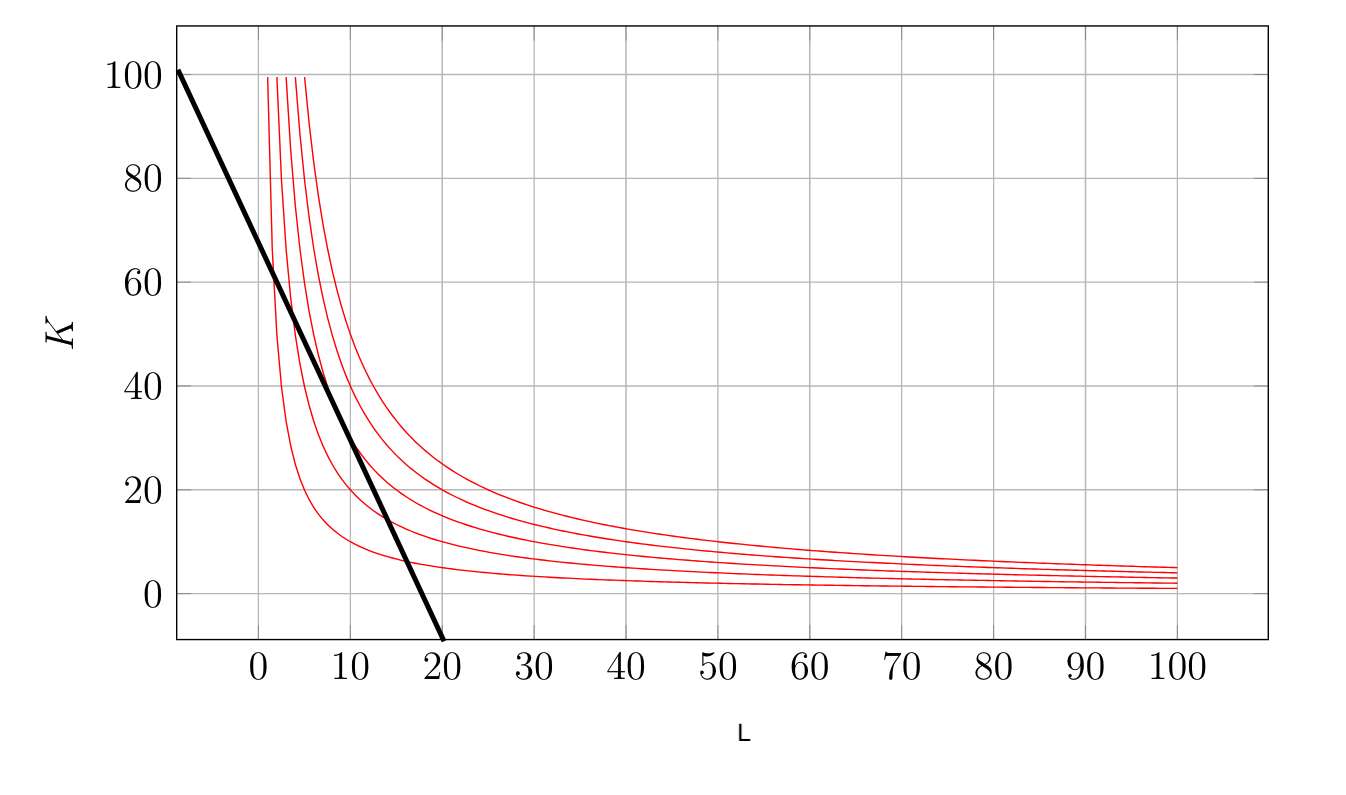
\includegraphics[width=\textwidth,height=10cm,keepaspectratio]{graph}
    \caption{Graphical maximization of Cobb-Douglas function}
    \label{fig:measurements}
\end{figure}

Clearly seen in the above figure, the constraint is tangent to the level curve when $C=300$, for a value of $L\approx 9$ and $C \approx 37$.







\subsection{Further scope and applications}
The concept of Lagrange Multiplier can also be used to optimize a host of other functions, of varying degrees. For example, it can be used for profit functions and other cost or production functions as well. Let there be a profit function defined as follows\footnote{McQuain, Margaret. \textit{Constrained Optimization: The Method of Lagrange Multipliers.} Virginia Tech, 2012, www.math.vt.edu/people/mcquain/1526\_Lag\_opt\_2012.pdf. Accessed on 19 Feb. 2019.} ,
\begin{equation}
	f(x,y)= -2x^2 +60x -3y^2 +72y +100
\end{equation}
where $x$ and $y$ are just two arbitrary products sold by a fictional company.

With a constraint,
\begin{equation}\label{eq:newconstraint}
	g(x,y)\Rightarrow x+y=20
\end{equation}

Just like in section \ref{sec:cobbdopt}, first the Lagrange equation must be made,
\begin{equation}
	L(x,y)=f(x,y)-\lambda g(x,y)
\end{equation}
Such that,
\begin{equation}
	-2x^2 +60x -3y^2 +72y +100 - \lambda (x+y-20)
\end{equation}
Finding the partial derivatives $P_x$,
\begin{equation}
	P_x \Rightarrow \frac{\partial}{\partial x}(-2x^2 +60x -3y^2 +72y +100)
\end{equation}
\begin{equation}
	\Rightarrow \frac{\partial}{\partial x}(-2x^2)+\frac{\partial}{\partial x}(60x)-\frac{\partial}{\partial x}(3y^2)+\frac{\partial}{\partial x}(72y)+\frac{\partial}{\partial x}(100)
\end{equation}
Since partial derivative with respect to $x$ for all $y$ terms is $0$,
\begin{equation}\label{eq:partialdforxnew}
	-4x+60=\lambda
\end{equation}
Similarly for $P_y$,
\begin{equation}\label{eq:ynew}
	P_y \Rightarrow -6y+72=\lambda
\end{equation}

Using \eqref{eq:partialdforxnew} and \eqref{eq:ynew} to get,
\begin{equation}
	x=15-\frac{1}{4}\lambda
\end{equation}
\begin{equation}
	y=12-\frac{1}{6}\lambda
\end{equation}
Solving system of equations with \eqref{eq:partialdforxnew}, \eqref{eq:ynew}, and \eqref{eq:newconstraint} by plugging in above values of $x$ and $y$ into \eqref{eq:newconstraint} of constraint=0,
\begin{equation}
	-x-y+20=-(15-\frac{1}{4}\lambda)-(12-\frac{1}{6}\lambda)+20
\end{equation}
\begin{equation}
	\Rightarrow -27 +\frac{10}{24}\lambda+20
\end{equation}
\begin{equation}
	\Rightarrow \lambda = \frac{-7\cdot 12}{5}
\end{equation}
Therefore, $\lambda=-16.8$ and $x \approx 10$ and $y \approx 9$ will produce the maximum profit under the constraints imposed. 

\newpage
\section{Conclusion and closing remarks}
Throughout this investigation, I was able to explore multivariable maximization using the Cobb-Douglas function through an algebraic and graphical outlook. Furthermore, I was able to apply the concepts of Lagrange Multipliers on more complicated functions, and maximize those as well. Although, my maximization techniques were limited to Lagrange Multipliers as well as graphical intuition. Furthermore, I set arbitrary constraints on real datasets that seem unlikely to work in real life. The constraints were set up the maximum cost that the function could incur when maximizing production. 

Nevertheless, I achieved the goal I initially sought out to achieve. I was able to take the dataset my father provided me and maximize the production for it. This deepened by belief in the applications of mathematics in economics. I was able to see how creating models and solving them are important for a firm, or any economic entity to succeed. 

This investigation could be furthered by maximizing various other functions. Many other price, cost, production, utility, etc. functions remain to be maximized. Maximizing production without constraints for more complicated functions wherein the marginal utility of production decreases would be beneficial to explore. Furthermore, maximizing more than two variables could also be helpful and interesting as many firms in today's day and age rarely rely on merely two factors of production in their production process.

Had my father and the IB Diploma Programme not shown me the relationship between mathematics and economics, I could never have completed this investigation. I gained an appreciation for the nuances between models and real-life situations as mathematics when applied on economics merely predicts the best-case scenario which is usually cofounded by multiple variables in real life. Regardless, I understood this relationship between these two fields on a deeper level, and I believe this investigation would be useful for my father's ventures as well.

Overall, I enjoyed this investigation and it taught me mathematical skills previously unknown, as well as the important lesson that what is predicted is often not the case when it comes to mathematics and models.


\newpage
\section{Works cited}
\singlespacing
\begin{flushleft}
\hangindent0.5in
\sloppy
\textbf{\large Print}

Amemiya, Takeshi. \textit{Advanced Econometrics.} Harvard University Press, 2001.

Beveridge, G. S. G., and R. S. Schechter. \textit{Optimization: Theory and Practice.} McGraw-Hill, 1970.

Coma, Charles W., and Paul H. Douglas. ``A theory of production." \textit{Proceedings of the Fortieth Annual Meeting of the American Economic Association,} vol. 139., 1928.

\textbf{\large Online}

Jingze, Jiang. ``How to Use Excel to Estimate the Cobb-Douglas Production Function." \textit{YouTube} 17 Apr. 2016, www.youtube.com/watch?v=FYHLc4zhjzg. Accessed on 10 Feb. 2019.

McQuain, Margaret. \textit{Constrained Optimization: The Method of Lagrange Multipliers.} Virginia Tech, 2012, www.math.vt.edu/people/mcquain/1526\_Lag\_opt\_2012.pdf. Accessed on 19 Feb. 2019.

\end{flushleft}
\end{document}


